\paragraph{Types of entities}

Three types of entities have been identified
\begin{itemize}
  \item \textit{Active}: an entity capable to start an action by itself,
  providing it the computational resources it needs;
  \item \textit{Reactive}: an entity with an inner state, that only acts on
reaction to external inputs, and it is not capable to start an action by itself;
  \item \textit{Passive}: an entity with an internal state (if necessary) which
is immutable. As a Reactive entity it only acts on reaction to external inputs,
and it is not capable to start an action by itself.
\end{itemize}

% \paragraph{Active}
% In light of the fact that active entities undertake spontaneous actions, in
% our context they are:
% \begin{itemize}
%   \item Moving entities: which move around the city according to their own
%     will;
%   \item Traffic lights: which autonomously change their color/state
%   by the time elapses.
% \end{itemize}

% \paragraph{Reactive}
% Streets (and all their parts) and crossroads should be reactive entities:
% \begin{itemize}
%   \item A street is used to travel towards a destination. It reacts to
%     travelers' inputs. Indeed it enables the travelers to move when they
%     walk or drive on it.
%     However, the state of a road is composed of the states of the reactive
%     sub-entities it comprises, e.g., stretches and houses;
%   \item A crossroads coordinates the traffic at street intersections
%     exclusively whenever a moving entity requires to cross it.
% \end{itemize}

% \paragraph{Passive}
% Passive entities are stateless. Therefore, road signs fit perfectly in this
% definition, since they represent immutable information that is read by road
% users.

\begin{table}[H]
\centering
\begin{tabular}{|l|l|}
\hline
\rowcolor{BlueGreen}
Type     & Entities                                 \\ \hline
Active   & pedestrian, bicycle, motorcycle, car, bus, traffic light \\ \hline
Reactive & road, crossroads, sidewalk, bike lane, crossing, house \\ \hline
Passive  & road signs                               \\ \hline
\end{tabular}
\caption{Types of entities}
\label{tab:entity_type}
\end{table}
Entity types have the following dependencies:
\begin{itemize}
  \item \textit{Active} entities provides inputs to the \textit{Reactive}
entities (solid line);
  \item \textit{Active} and \textit{Reactive} entities can use \textit{Passive}
entities, the dependency is not strict (dashed line).
\end{itemize}
\begin{figure}[H]
  \centering
  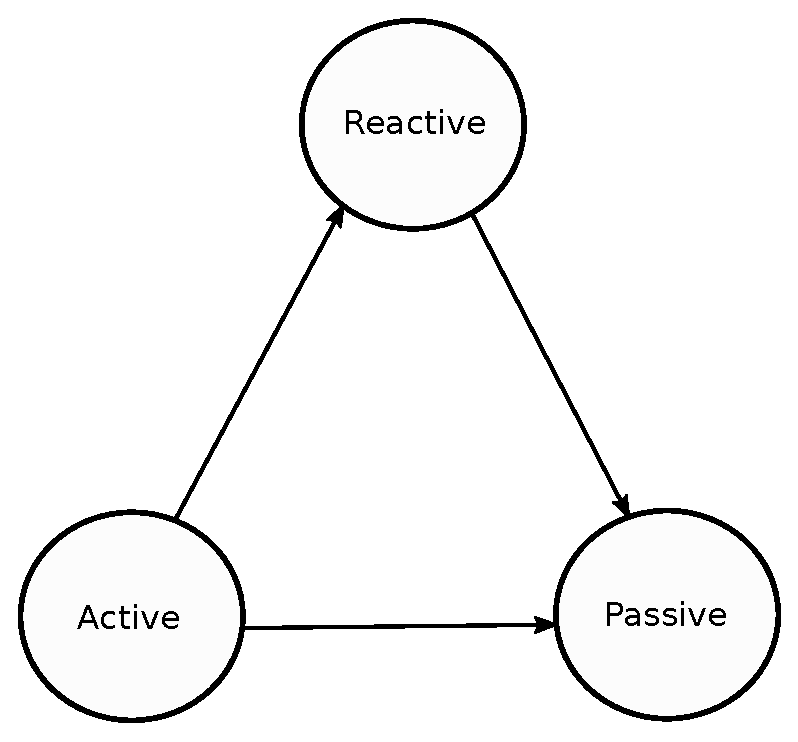
\includegraphics[width=.35\columnwidth]{images/solution/entity_type_dependency.eps}
  \caption{Dependencies between entity types}
  \label{fig:sd-entity-types-deps}
\end{figure}
